\documentclass[a4paper,12pt]{article}
\usepackage{graphicx}
\usepackage{hyperref}
\usepackage{caption}

\title{Exposé: Analyse von GovTech-Institutionen und ihren Netzwerken}
\author{Robin Dörnemann}
\date{\today}

\begin{document}

\maketitle

\section{Einleitung}
Dieses Projekt zielt darauf ab, die Netzwerke und Verbindungen von GovTech-Startups zu analysieren, einschließlich ihrer Beziehungen zu anderen Akteuren wie Behörden, anderen Startups und Institutionen. Durch die Pflege einer umfassenden Datenbank, die alle GovTech-Startups und ihre Gründer enthält, soll ein tieferes Verständnis der GovTech-Landschaft und ihrer dynamischen Interaktionen gewonnen werden.

\section{Ziele}
\subsection*{Analyse der GovTech-Verbindungen}
Das Hauptziel des Projekts ist es, die Verbindungen zwischen GovTech-Startups und anderen Akteuren auf LinkedIn zu identifizieren und zu analysieren. Dies umfasst die Untersuchung der Netzwerke, die GovTech-Unternehmen durch ihre LinkedIn-Verbindungen mit Behörden, anderen Startups und Institutionen aufbauen. Dabei wird analysiert, wie diese Verbindungen genutzt werden, um Kooperationen zu fördern, Wissen auszutauschen und strategische Partnerschaften zu entwickeln.

\subsection*{Aufbau einer umfassenden GovTech-Datenbank}
Ein weiteres Ziel ist die Erstellung und Pflege einer detaillierten Datenbank, die Informationen über GovTech-Startups und ihre Gründer sammelt. Diese Datenbank dient als zentrale Ressource zur Unterstützung der Analyse und zur Bereitstellung wertvoller Einblicke in die Struktur und Entwicklung der GovTech-Industrie.

\subsection*{Netzwerkzentralität und Einflussanalyse}
Durch die Analyse der Netzwerkzentralität soll das Projekt einflussreiche Akteure innerhalb des GovTech-Ökosystems identifizieren. Diese Erkenntnisse sind entscheidend für das Verständnis von Machtstrukturen und der potenziellen Auswirkungen auf die Entwicklung und Umsetzung von GovTech-Initiativen.

\subsection*{Visualisierung der Netzwerke}
Das Projekt plant die Entwicklung von Visualisierungen, die die komplexen Beziehungen und Interaktionen innerhalb des GovTech-Ökosystems veranschaulichen.

\section{Methodik}
\subsection*{Technologischer Stack}
Das Projekt nutzt einen umfassenden technologischen Stack, um die Analyse der LinkedIn-Verbindungen von GovTech-Startups effizient durchzuführen. Der \textbf{Python Scraper} wird entwickelt, um relevante Daten effizient von LinkedIn zu extrahieren. Diese Daten werden in einer \textbf{PostgreSQL-Datenbank} gespeichert, die zur Verwaltung und Organisation der gesammelten Informationen dient. \textbf{FastAPI} wird eingesetzt, um eine leistungsfähige API für den Datenzugriff und die Manipulation bereitzustellen. Zur Sicherstellung einer konsistenten Entwicklungsumgebung und zur Erleichterung der Bereitstellung wird \textbf{Docker} verwendet.

\subsection*{Visualisierungstools}
Für die Visualisierung der Analyseergebnisse werden verschiedene Tools eingesetzt. \textbf{Plotly/Dash} wird verwendet, um interaktive Diagramme zu erstellen, die die Analyseergebnisse veranschaulichen. \textbf{NetworkX} dient zur Darstellung von Netzwerkgrafiken, die die Beziehungen zwischen den Akteuren visualisieren. \textbf{D3.js} ermöglicht anpassbare Visualisierungen, die spezifische Datenanalysen unterstützen und detaillierte Einblicke in die Netzwerkstrukturen bieten.

\section{Ergebnisse}
\subsection*{Geplante Visualisierungen}
Die Visualisierungen sind ein zentraler Bestandteil des Projekts. Sie bieten eine intuitive Darstellung der Analyseergebnisse und helfen, komplexe Datenmuster zu erkennen und zu interpretieren.

\begin{figure}[h]
    \centering
    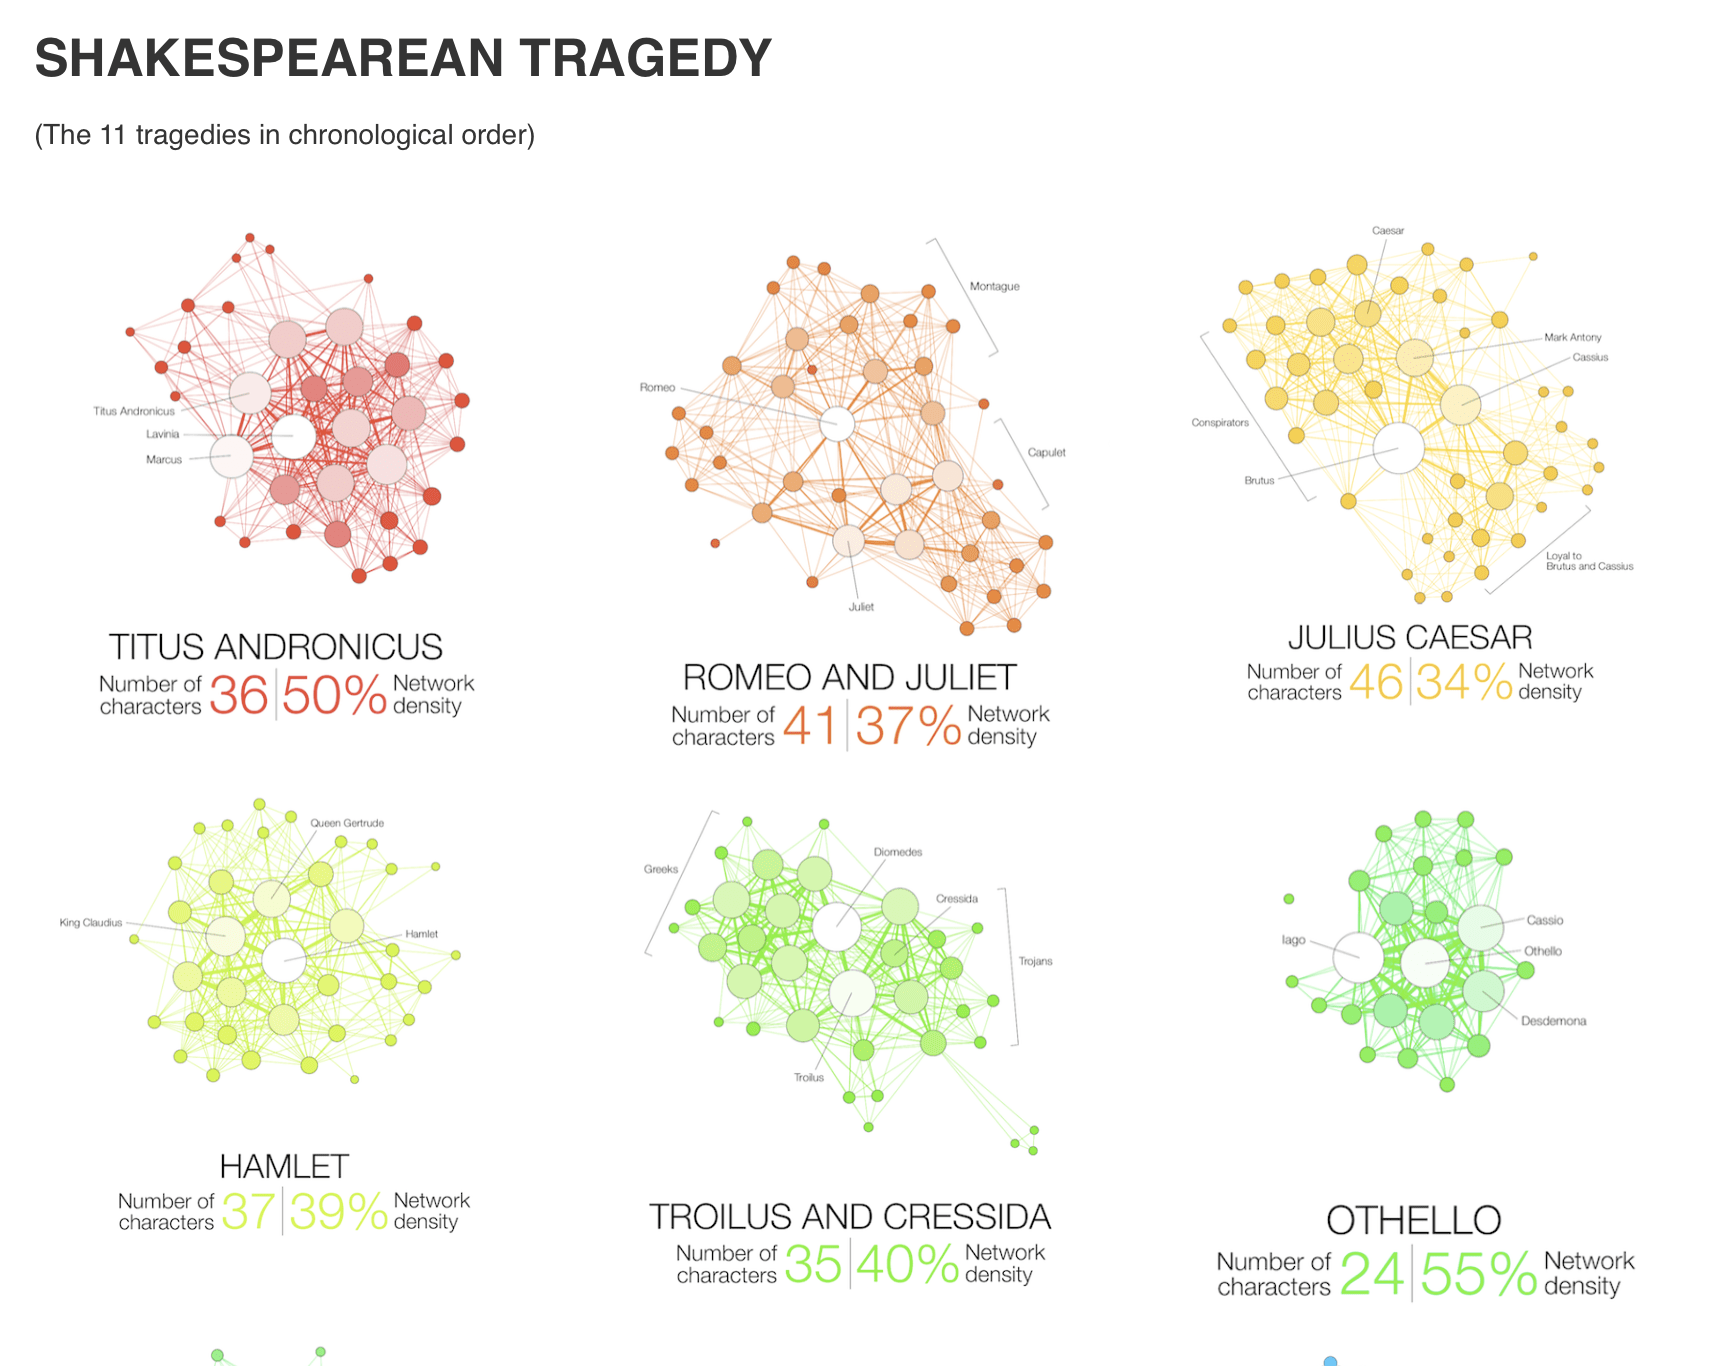
\includegraphics[width=0.8\textwidth]{net.png}
    \caption{Demo für Diagramm der GovTech-Verbindungen}
\end{figure}

\section{Zeitplan und Ressourcen}
\subsection*{Zeitrahmen}
Das Projekt ist auf einen Zeitraum von wenigen Wochen ausgelegt.

\subsection*{Benötigte Ressourcen}

Falls möglich kann der Scraper von Dr. G integriert werden.



\end{document}

